\documentclass[a4paper,fleqn]{cas-sc}

% Elsevier CAS template; target journal: Simulation Modelling Practice and Theory.
\usepackage[T1]{fontenc}
\usepackage[utf8]{inputenc}
\usepackage[english]{babel}
\usepackage[authoryear]{natbib}
\usepackage{amsmath,amssymb}
\usepackage{graphicx}
\usepackage{booktabs}
\usepackage{array}
\usepackage{float}
\usepackage{xcolor}
\usepackage{microtype}
\microtypesetup{expansion=false}
\IfFileExists{xurl.sty}{\usepackage{xurl}}{\usepackage{url}}
\setlength{\emergencystretch}{3em}
\hyphenation{inter-community intra-community Gillespie}

\floatstyle{ruled}
\newfloat{algorithm}{tbp}{loa}
\floatname{algorithm}{Algorithm}
\floatstyle{plain}
\restylefloat{figure}
\restylefloat{table}

\newtheorem{proposition}{Proposition}
\newtheorem{corollary}{Corollary}
\newdefinition{remark}{Remark}
\newproof{proof}{Proof}

\newcommand{\ibar}{\bar{y}}
\newcommand{\sbar}{\bar{s}}
\newcommand{\Exp}{\mathrm{Exp}}
\newcommand{\Full}{\textup{\textsc{Full}}}
\newcommand{\TS}{\textup{\textsc{TwoScale}}}
\newcommand{\ind}{\mathbf{1}}
\newcommand{\eW}{e_{W}}

\begin{document}
\let\WriteBookmarks\relax
\def\floatpagepagefraction{1}
\def\textpagefraction{.001}

\shorttitle{Two-scale stochastic simulation with aggregate inter-community coupling}
\shortauthors{Y. Kuryliak and M.T.M. Emmerich}

\title[mode=title]{Two-scale stochastic simulation of epidemics on community networks: formulation and accuracy of aggregate inter-community coupling}

\author[1]{Yulian Kuryliak}[orcid=0000-0002-6600-2637]
\cormark[1]
\ead{yulian.a.kuryliak@lpnu.ua}
\affiliation[1]{organization={Institute of Computer Science and Information Technologies, Lviv Polytechnic National University},
            addressline={12 Stepan Bandera Street},
            city={Lviv},
            postcode={79000},
            country={Ukraine}}

\author[2]{Michael T. M. Emmerich}[orcid=0000-0002-7342-2090]
\ead{michael.t.m.emmerich@jyu.fi}
\affiliation[2]{organization={Faculty of Information Technology, University of Jyv\"askyl\"a},
            addressline={P.O. Box 35 (Agora)},
            city={Jyv\"askyl\"a},
            postcode={FI-40014},
            country={Finland}}

\cortext[1]{Corresponding author}

\begin{abstract}
Epidemic simulations of structured populations often combine detailed contact networks within communities with only aggregate information about contacts between them. We study a two-scale stochastic simulator for this setting, previously outlined in a workshop paper: each community is simulated exactly by its own Gillespie engine, while inter-community infections are timed by aggregate, state-dependent hazards and placed uniformly among susceptible nodes of the receiving community. We give a complete specification of the method, including its grid-based synchronisation, and show that its ideal version is an exact simulation of a surrogate network in which each bundle of inter-community edges is replaced by uniform all-to-all coupling of equal total weight. This representation identifies four sources of discrepancy (lost boundary-state information, uniform placement, absent exhaustion of interface edges and synchronisation error) and implies that, for randomly placed interfaces, the ideal aggregate export clock is stochastically earlier than the full-network one. We compared the method with full-network Gillespie simulation of SI dynamics in single-export benchmarks and in 48 configurations of ten-community chains (50--1000 nodes per community, internal path lengths 1--6, one or five interface edges, 400 matched runs each). When the spread of infection times within a community was below a quarter of the mean single-edge crossing time, terminal arrival-time distributions were statistically indistinguishable in 15 of 18 configurations; beyond this, the two-scale simulator arrived early by an amount roughly proportional to that ratio, reaching 40\%. Close timing did not imply admissible routes: up to 52\% of aggregate crossings preceded infection of any true bridge node.
\end{abstract}

\begin{highlights}
\item Exact local Gillespie engines are coupled through aggregate inter-community hazards
\item The ideal scheme is exact simulation of a surrogate all-to-all interface network
\item Aggregate export clocks are stochastically early for randomly placed interfaces
\item Accuracy is organised by internal timing spread relative to edge crossing time
\item Close arrival times can coexist with physically impossible transmission routes
\end{highlights}

\begin{keywords}
Stochastic simulation \sep Gillespie algorithm \sep Multiscale simulation \sep Community networks \sep Epidemic modelling \sep Approximation error
\end{keywords}

\maketitle

%======================================================================
\section{Introduction}
\label{sec:introduction}

The contact structure of a population shapes how an infection spreads: heterogeneous and clustered contacts change epidemic thresholds, growth and arrival times relative to homogeneous mixing \citep{keeling2005,pastorsatorras2015,kiss2017}. At larger scales, transmission between cities or regions is driven by mobility, which is usually described by flows between locations rather than by individual contacts \citep{balcan2009,barbosa2018human}. Models of such systems therefore face information at two resolutions. Inside a community, a contact network may be observed, reconstructed or synthesised \citep{eubank2004,danon2011}. Between communities, often only aggregate quantities such as commuting volumes or mobility counts are available \citep{barbosa2018human,chang2021}.

If the complete contact network were known, the epidemic would be a continuous-time Markov chain (CTMC) that can be sampled exactly by Gillespie-type algorithms \citep{gillespie1977exact,gibson2000}, and efficient network implementations make this feasible for large graphs \citep{vestergaard2015,kuryliak2025simulating}. Exact simulation, however, requires every transmission channel to be specified, including each contact between communities. Metapopulation models take the opposite approach: they operate on aggregate flows but also replace the within-community dynamics by compartments \citep{colizza2007reaction,colizza2008,balcan2010modeling,ajelli2010}. Between these extremes lies a practically relevant intermediate model, in which detailed stochastic network dynamics are retained inside communities and only the interface between communities is aggregated.

A two-scale simulator of this kind was outlined in a short workshop paper \citep{kuryliak2025towards}. Each community is simulated by its own exact Gillespie engine; a macro layer generates inter-community infections from aggregate rates that depend on the current infected and susceptible fractions of the communities, and each imported infection is placed in the receiving community. The workshop paper motivated the architecture by the cost of representing every inter-community contact and sketched its layers; it left the analysis of the error introduced by aggregation as the next step. Because that description was brief, we present the method here in a self-contained form.

The central question of this article is how accurately the aggregate interface reproduces the full-network CTMC that it replaces, for which observables and in which network regimes. The answer depends on the information that the interface discards: which nodes actually carry the interface, where an imported infection lands, and how often a thin interface can be crossed. We address it analytically and by controlled simulation experiments in which the complete network is known to the experimenter but only its aggregate representation is passed to the two-scale simulator.

The contributions are as follows.
\begin{enumerate}
\item A complete, implementation-level specification of the two-scale method, including the grid-synchronised hazard-integral scheduler used in practice (Section~\ref{sec:method}, Algorithm~\ref{alg:scheduler}).
\item An exact characterisation of the ideal method as full-network simulation on a surrogate network with uniform all-to-all interface coupling (Proposition~\ref{prop:surrogate}). It yields a taxonomy of discrepancies and a stochastic-ordering result for single exports (Proposition~\ref{prop:ordering}).
\item A controlled comparison with full-network Gillespie simulation on single-export benchmarks and on chains of communities, using permutation baselines that separate approximation error from sampling variability (Sections~\ref{sec:design} and~\ref{sec:results}).
\item A practical criterion: the ratio of the within-community spread of infection times to the single-edge crossing time organises the observed discrepancies across community sizes, internal structures and interface widths (Section~\ref{sec:res_descriptor}).
\end{enumerate}

The study is restricted to susceptible--infected (SI) dynamics on static synthetic networks and a fixed synchronisation step. Section~\ref{sec:related} relates the method to existing simulation approaches; Section~\ref{sec:method} specifies it; Section~\ref{sec:analysis} analyses what the aggregate interface preserves; Sections~\ref{sec:design} and~\ref{sec:results} describe the experiments and their results; Section~\ref{sec:discussion} discusses practical use, cost and limitations.

%======================================================================
\section{Related work}
\label{sec:related}

\paragraph{Exact and approximate stochastic simulation.}
Gillespie's direct method samples a CTMC exactly from the current propensities \citep{gillespie1977exact}; the next reaction method organises the same computation around per-channel clocks \citep{gibson2000}. When propensities vary in time, exact simulation can be expressed through the random-time-change representation of a counting process \citep{ethier1986}: an event fires when its integrated intensity reaches an independent exponential threshold. \citet{anderson2007} turned this representation into the modified next reaction method for time-dependent propensities. The macro clock of the two-scale simulator is an instance of this construction with a stochastic, state-dependent intensity. Network-oriented implementations update only the propensities affected by an event \citep{vestergaard2015,kuryliak2025simulating}; the local engines used here follow \citet{kuryliak2025simulating}.

Hybrid and multiscale stochastic simulation algorithms accelerate systems with widely separated reaction rates by approximating fast channels \citep{haseltine2002,cao2005slow}. The two-scale method differs in what it approximates: it does not average fast channels but removes information about which inter-community channels are active. As shown in Section~\ref{sec:results}, its accuracy is nevertheless organised by a separation of time scales, namely between internal spread and interface crossing.

\paragraph{Metapopulation and mobility models.}
Metapopulation models couple subpopulations through mobility flows and have been used to study invasion thresholds and global spread \citep{colizza2007reaction,colizza2008,balcan2009,balcan2010modeling}; mobility networks of high resolution can be combined with local transmission models \citep{chang2021}. Agent-based models resolve individuals throughout \citep{eubank2004,kerr2021}, and \citet{ajelli2010} compared the two paradigms. The two-scale method keeps individual nodes and contacts inside communities, so that local stochasticity and network structure are preserved, while it uses only metapopulation-type information between communities.

\paragraph{Two levels of mixing and co-simulation.}
Epidemic models with two levels of mixing combine local contacts within small groups with uniform global mixing \citep{ball1997}. The surrogate network of Proposition~\ref{prop:surrogate} has the same structure, with global mixing restricted to pairs of communities and weighted by the aggregate coupling. From a simulation-engineering perspective, the two-scale scheduler is a co-simulation master that advances black-box subsystems on a communication grid and exchanges a few coupling variables \citep{gomes2018cosim}. Unlike typical co-simulation interfaces, the interface here does not only transfer state; it also defines when and where stochastic events occur in the receiving subsystem.

%======================================================================
\section{The two-scale simulation method}
\label{sec:method}

\subsection{Full-network reference model}
\label{sec:reference}

Let $G=(V,E)$ be a contact network whose node set is partitioned into $M$ communities, $V=\bigsqcup_{i=1}^{M}V_i$, with $N_i=|V_i|$. We treat $E$ as a set of oriented transmission channels; an undirected contact contributes two channels. The channels are divided into within-community bundles $E_{ii}$ and inter-community bundles $E_{ij}=\{(u,v)\in E:u\in V_i,\,v\in V_j\}$, $i\neq j$. Each node is susceptible ($S$), infected ($I$) or removed ($R$). For a configuration $x\in\{S,I,R\}^V$, let $x^{v:I}$ and $x^{u:R}$ denote the configurations in which node $v$ has become infected or node $u$ has been removed. The full-network process is the CTMC with generator
\begin{equation}
\label{eq:full_generator}
(\mathcal{L}_G f)(x)=\sum_{(u,v)\in E}\beta_{uv}\,\ind\{x_u=I,\,x_v=S\}\bigl[f(x^{v:I})-f(x)\bigr]
+\sum_{u\in V}\gamma\,\ind\{x_u=I\}\bigl[f(x^{u:R})-f(x)\bigr],
\end{equation}
where $\beta_{uv}$ is the transmission rate of channel $(u,v)$ and $\gamma$ the removal rate. Inter-community rates are written as $\beta_{uv}=\beta_{\mathrm{out}}w_{uv}$ with contact weights $w_{uv}$. We call the exact simulation of~\eqref{eq:full_generator} \Full{}. All experiments in this article use SI dynamics ($\gamma=0$).

\subsection{Aggregate interface}
\label{sec:interface}

The two-scale simulator, denoted \TS{}, receives the within-community graphs $G_i=(V_i,E_{ii})$ with their rates, but not the inter-community bundles. Each bundle is represented only by its aggregate weight
\begin{equation}
\label{eq:weight}
W_{ij}=\sum_{(u,v)\in E_{ij}}w_{uv},\qquad i\neq j,
\end{equation}
which for unit weights is the number of channels from $V_i$ to $V_j$. In applications, $W_{ij}$ would be estimated from mobility or contact surveys rather than computed from a known network. The state of community $i$ is summarised by its counts $s_i$ and $y_i$ of susceptible and infected nodes and the corresponding fractions $\sbar_i=s_i/N_i$ and $\ibar_i=y_i/N_i$. Table~\ref{tab:information} lists the information used by each model. Figure~\ref{fig:schematic}(a,b) contrasts the two representations.

\begin{table}[tbp]
\centering
\caption{Information used by the full-network reference and by the two-scale simulator.}
\label{tab:information}
\small
\begin{tabular}{>{\raggedright\arraybackslash}p{0.38\linewidth}>{\raggedright\arraybackslash}p{0.25\linewidth}>{\raggedright\arraybackslash}p{0.27\linewidth}}
\toprule
Item & \Full{} & \TS{}\\
\midrule
Within-community contacts and rates & yes & yes\\
Node states within communities & yes & yes (local engines)\\
Inter-community channels $E_{ij}$ (bridge nodes and endpoints) & yes & no\\
Aggregate weight $W_{ij}$ & implied by $E_{ij}$ & yes\\
Rate of transmission from $V_i$ to $V_j$ & from states of channels in $E_{ij}$ & from $\ibar_i$, $\sbar_j$ and $W_{ij}$\\
Receiving node of a transmission & endpoint of the firing channel & drawn from a placement rule\\
Maximum transmissions across a bundle (SI) & number of channels & limited only by $s_j$\\
\bottomrule
\end{tabular}
\end{table}

\begin{figure}[tbp]
\centering
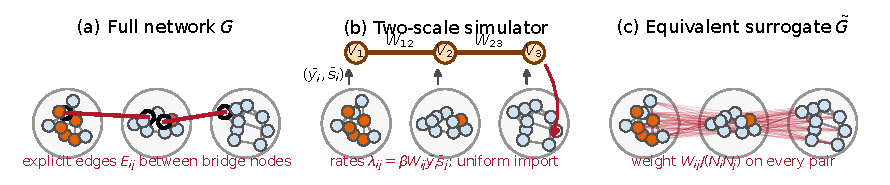
\includegraphics[width=\linewidth]{Images/twoscale/fig_method_schematic.pdf}
\caption{(a) Full network: infection crosses between communities only along explicit edges joining bridge nodes (black rings). (b) Two-scale simulator: each community is an exact local Gillespie engine; the macro layer sees only the fractions $(\ibar_i,\sbar_i)$ and the aggregate weights $W_{ij}$, generates inter-community infections at rates $\lambda_{ij}$ and places each import on a uniformly chosen susceptible node. (c) The equivalent surrogate network of Proposition~\ref{prop:surrogate}: every pair of nodes in adjacent communities is joined by a weak edge of weight $W_{ij}/(N_iN_j)$. Orange: infected; blue: susceptible.}
\label{fig:schematic}
\end{figure}

\subsection{Local engines}
\label{sec:local}

Each community is simulated by a separate engine that samples the CTMC of its own graph $G_i$: infection along channels in $E_{ii}$ and removal of infected nodes, with the propensities of~\eqref{eq:full_generator} restricted to $V_i$. The engines use the incremental Gillespie implementation of \citet{kuryliak2025simulating}, in which each node stores the weight of its contacts with infected neighbours and only the propensities affected by an event are updated. Each engine owns a private pseudorandom stream.

An engine supports two operations used by the macro layer: advancing its clock to a prescribed time, applying only the events that occur before it, and an \emph{import}, which sets a given susceptible node to $I$. An import changes the local propensities; the engine therefore discards its pending next event and samples a new one from the updated state. Because the waiting times of a CTMC are memoryless, this restart preserves the law of the local process. Between imports, each engine is an exact simulation of its community in isolation.

\subsection{Macro layer}
\label{sec:macro}

The macro layer treats communities as nodes of a weighted graph with weights $W_{ij}$. Given the current summaries, it assigns to every ordered pair $i\neq j$ the hazard
\begin{equation}
\label{eq:macro_rate}
\lambda_{ij}(t)=\beta_{\mathrm{out}}\,W_{ij}\,\ibar_i(t)\,\sbar_j(t),
\qquad
\Theta(t)=\sum_{i\neq j}\lambda_{ij}(t).
\end{equation}
A macro event is a single infection transmitted from some community to another. When it occurs, the pair $(i,j)$ is selected with probability $\lambda_{ij}/\Theta$, and a target $v\in S_j$ is drawn from a placement rule $\Pi_{ij}(\cdot\mid x)$. The default rule, used throughout this article, is uniform placement, $\Pi_{ij}(v\mid x)=1/s_j$. Degree-weighted or boundary-aware rules are possible when such information is available. The implementation also contains a multiplicative calibration factor for~\eqref{eq:macro_rate}, which was set to one.

Given the community counts, rate~\eqref{eq:macro_rate} is the expected rate of the bundle $E_{ij}$ when its endpoints are placed uniformly at random. It coincides with the actual rate when the bundle joins every pair of nodes with equal weight (Corollary~\ref{cor:exact}) and is an approximation otherwise (Section~\ref{sec:analysis}). The macro layer is not autonomous: $\Theta$ changes whenever a local event or an import changes a community count. Because the summaries are piecewise constant between such events, so is $\Theta$.

\subsection{Hazard-integral timing and synchronisation}
\label{sec:timing}

Let $t_0$ be the time of the previous macro event and $E\sim\Exp(1)$ an independent threshold. In the ideal construction, the next macro event occurs at
\begin{equation}
\label{eq:hazard_integral}
t^\ast=\inf\Bigl\{t>t_0:\int_{t_0}^{t}\Theta(s)\,ds\ge E\Bigr\},
\end{equation}
which is the random-time-change representation of a counting process with intensity $\Theta$ \citep{ethier1986,anderson2007}. For constant $\Theta$ it reduces to Gillespie's waiting time $(t^\ast-t_0)=-\ln U/\Theta$, $U\sim\mathcal{U}(0,1)$. Combined with exact local engines, construction~\eqref{eq:hazard_integral} defines the \emph{ideal} two-scale process, whose transition rates are given in Section~\ref{sec:surrogate}.

The implemented scheduler (Algorithm~\ref{alg:scheduler}) treats the local engines as black boxes that expose their state only when they are advanced. It divides time into synchronisation intervals of length $\tau$ and estimates $\Theta$ on each (sub)interval $[t,t_g)$ by a midpoint probe: copies of all engines, including the states of their random-number generators, are advanced to $t+\Delta/2$, where $\Delta=t_g-t$, and $\Theta_{\mathrm{mid}}$ is computed from the copies. If the accumulated hazard $A+\Theta_{\mathrm{mid}}\Delta$ stays below $E$, the actual engines are advanced to $t_g$. Otherwise, the crossing time is interpolated as
\begin{equation}
\label{eq:interpolation}
t^\ast=t+\frac{E-A}{\Theta_{\mathrm{mid}}},
\end{equation}
the engines are advanced to $t^\ast$, and the pair and the target are sampled from their states at $t^\ast$. The threshold is then renewed and the remainder of the interval is processed in the same way.

\begin{algorithm}[tbp]
\caption{Grid-synchronised two-scale simulation of one realisation.}
\label{alg:scheduler}
\small
\begin{tabbing}
\hspace*{1.6em}\=\hspace*{1.4em}\=\hspace*{1.4em}\=\hspace*{1.4em}\=\kill
\textbf{Input:} local graphs $G_i$, weights $W_{ij}$, rates, step $\tau$, horizon $T_{\mathrm{end}}$, initial state.\\[2pt]
1:\> $t\gets 0$;\ \ $A\gets 0$;\ \ draw $E\sim\Exp(1)$\\
2:\> \textbf{while} $t<T_{\mathrm{end}}$ and infection can still spread \textbf{do}\\
3:\>\> $t_g\gets\min(t+\tau,\,T_{\mathrm{end}})$\\
4:\>\> \textbf{while} $t<t_g$ \textbf{do}\\
5:\>\>\> $\Delta\gets t_g-t$; copy every engine with its random-number state; advance the copies to $t+\Delta/2$\\
6:\>\>\> $\Theta_{\mathrm{mid}}\gets\sum_{i\neq j}\lambda_{ij}$ evaluated on the copies, Eq.~\eqref{eq:macro_rate}\\
7:\>\>\> \textbf{if} $A+\Theta_{\mathrm{mid}}\Delta<E$ \textbf{then} \hspace{1em}{\color{black!60}// no macro event before $t_g$}\\
8:\>\>\>\> advance all engines to $t_g$;\ \ $A\gets A+\Theta_{\mathrm{mid}}\Delta$;\ \ $t\gets t_g$\\
9:\>\>\> \textbf{else}\\
10:\>\>\>\> $t^\ast\gets t+(E-A)/\Theta_{\mathrm{mid}}$;\ \ advance all engines to $t^\ast$\\
11:\>\>\>\> sample $(i,j)$ with probability $\lambda_{ij}(t^\ast)/\Theta(t^\ast)$ from the engines' states\\
12:\>\>\>\> draw $v$ uniformly from $S_j(t^\ast)$; import $v$ into engine $j$ (its pending event is discarded)\\
13:\>\>\>\> $t\gets t^\ast$;\ \ $A\gets 0$;\ \ draw a new $E\sim\Exp(1)$
\end{tabbing}
\end{algorithm}

Two properties of the scheduler matter for interpreting the results. First, because the probes copy the random-number states, a probe reproduces the trajectory that the corresponding engine will actually follow up to the midpoint, unless an import intervenes. The midpoint rule is therefore a quadrature of the realised piecewise-constant hazard. It is exact on subintervals without local events in any community, and its error and its look-ahead of at most $\tau/2$ vanish as $\tau\to0$. Second, when the local engines expose their event times, the black-box assumption is unnecessary. Since $\Theta$ is piecewise constant between local events, integral~\eqref{eq:hazard_integral} can then be evaluated exactly by an event-driven scheduler that merges the next-event times of all engines. This removes the synchronisation error altogether. We evaluate the grid-based variant, which is the one implemented, with $\tau=1$.

\subsection{Computational structure and intended use}
\label{sec:cost}

\Full{} stores every channel, including all inter-community channels, and its cost per event grows with node degree \citep{kuryliak2025simulating}. \TS{} stores the within-community graphs and an $M\times M$ weight matrix. This is the saving emphasised in the workshop paper \citep{kuryliak2025towards}: when inter-community contacts are numerous, for example when a mobility flow corresponds to many individual contacts, the interface reduces to $O(M^2)$ numbers. Local engines can also be modified independently, which makes community-specific interventions straightforward to represent. Against this, the grid-synchronised scheduler adds a cost proportional to $(T_{\mathrm{end}}/\tau)\sum_iN_i$ for copying engine states, independent of the number of events. The method is therefore suited to settings in which the inter-community contacts are unknown or too numerous to represent, rather than to small networks whose full contact structure is available. Measured run times are reported in Section~\ref{sec:disc_cost}.

%======================================================================
\section{What the aggregate interface preserves and what it loses}
\label{sec:analysis}

\subsection{Surrogate-network representation}
\label{sec:surrogate}

With exact timing~\eqref{eq:hazard_integral}, the ideal two-scale process is a CTMC on $\{S,I,R\}^V$. Its rate of the transition $x\to x^{v:I}$ by an import is $\sum_{i\neq j}\lambda_{ij}(x)\Pi_{ij}(v\mid x)$ for $v\in S_j(x)$; all local transitions have the rates of~\eqref{eq:full_generator} restricted to $E_{ii}$. The following proposition identifies this process with a full-network process on a modified graph.

\begin{proposition}[Surrogate network]
\label{prop:surrogate}
Let $\tilde G$ be the network with the same within-community channels and rates as $G$, in which every inter-community bundle $E_{ij}$ is replaced by the complete set of channels $V_i\times V_j$, each with rate $\tilde\beta_{uv}=\beta_{\mathrm{out}}W_{ij}/(N_iN_j)$. Under uniform placement, the ideal two-scale process has generator $\mathcal{L}_{\tilde G}$; that is, it has the law of the full-network process on $\tilde G$ started from the same configuration.
\end{proposition}

\begin{proof}
Removals and within-community infections have identical rates in both processes. Consider a susceptible node $v\in V_j$ in configuration $x$. Under uniform placement, the two-scale rate at which $v$ is infected by an import is
\[
\sum_{i\neq j}\lambda_{ij}(x)\,\frac{1}{s_j(x)}
=\sum_{i\neq j}\beta_{\mathrm{out}}W_{ij}\frac{y_i(x)}{N_i}\frac{s_j(x)}{N_j}\frac{1}{s_j(x)}
=\sum_{i\neq j}\sum_{u\in V_i}\frac{\beta_{\mathrm{out}}W_{ij}}{N_iN_j}\ind\{x_u=I\},
\]
which is the total rate of the inter-community channels of $\tilde G$ that point into $v$. When $s_j(x)=0$ both rates vanish. Hence all transition rates coincide and the generators are equal. \qed
\end{proof}

\begin{corollary}
\label{cor:exact}
If every inter-community bundle of $G$ is already complete, $E_{ij}=V_i\times V_j$, with a common rate per pair of communities, then $\tilde G=G$ and the ideal two-scale process is exact.
\end{corollary}

The surrogate preserves the total weight of every bundle, $\sum_{(u,v)\in V_i\times V_j}\tilde\beta_{uv}=\beta_{\mathrm{out}}W_{ij}$, but spreads it uniformly over all pairs (Figure~\ref{fig:schematic}c). The approximation error of the ideal method is therefore the difference between epidemics on $G$ and on $\tilde G$, which differ only in their interfaces. The implemented method adds a numerical synchronisation error. Proposition~\ref{prop:surrogate} also provides a practical verification route: for small networks, the synchronisation error can be isolated by comparing the two-scale simulator with exact simulation on $\tilde G$.

\subsection{Sources of discrepancy}
\label{sec:sources}

Comparing $G$ with $\tilde G$ gives four mechanisms by which the two-scale simulator can depart from the full-network process.

\paragraph{Boundary-state information (source side).}
In $G$, the rate of transmission from $V_i$ to $V_j$ is
\begin{equation}
\label{eq:exact_rate}
a^\star_{ij}(x)=\beta_{\mathrm{out}}\sum_{(u,v)\in E_{ij}}w_{uv}\,\ind\{x_u=I,\,x_v=S\},
\end{equation}
which depends on whether the particular bridge nodes are infected. In $\tilde G$, every infected node of $V_i$ contributes. Exports can therefore occur before any bridge node is infected. Such \emph{bridge bypass} is impossible in $G$ and provides a direct diagnostic (Section~\ref{sec:single_export}).

\paragraph{Placement (receiver side).}
In $G$, a transmission infects the target endpoint of the firing channel; in $\tilde G$, the target is uniform among susceptible nodes. The location of an import determines its distance to the next interface and hence later crossings.

\paragraph{Interface exhaustion (receiver side).}
Under SI dynamics, a channel of $G$ transmits at most once: afterwards its target is infected. A bundle with $|E_{ij}|$ channels therefore carries at most $|E_{ij}|$ transmissions, and a single-edge interface exactly one. In $\tilde G$, imports from $V_i$ into $V_j$ continue at rate $\lambda_{ij}=\beta_{\mathrm{out}}W_{ij}\ibar_i\sbar_j$ until $V_j$ is exhausted; their expected number over a period $[t_1,t_2]$ is $\mathbb{E}\int_{t_1}^{t_2}\lambda_{ij}(s)\,ds$. When a receiving community remains largely susceptible for a long time, the two-scale simulator therefore keeps seeding it with additional infections that the full network cannot deliver.

\paragraph{Synchronisation.}
The midpoint quadrature and interpolation of Section~\ref{sec:timing} approximate~\eqref{eq:hazard_integral}.

\begin{remark}[Placement under randomised interfaces]
\label{rem:placement}
Suppose that the endpoints of each bundle are sampled uniformly and independently of the internal graphs and of the endpoints of other bundles, as in the experiments below. Then the target of the first transmission into a fully susceptible community is uniformly distributed in $G$, because it is the endpoint of a uniformly placed channel, and also in $\tilde G$. Placement can therefore affect arrival times only through transmissions after the first. In such designs, differences between the first crossing and later crossings isolate receiver-side effects (Section~\ref{sec:res_descriptor}).
\end{remark}

\subsection{Single export: stochastic ordering and bridge bypass}
\label{sec:single_export}

Consider a source community $V_0$ of size $n$ with an arbitrary internal graph, SI dynamics, and a single susceptible leaf node $\ell$ joined to a set $B\subset V_0$ of $k$ bridge nodes by channels of rate $\beta_{\mathrm{out}}$. Then $W_{0\ell}=k$, and before the export $\sbar_\ell=1$, so that $\lambda_{0\ell}=\beta_{\mathrm{out}}k\,\ibar_0$. Let $\tau_u$ be the infection time of node $u$, $A_u(t)=(t-\tau_u)^+$ its infection age, and $T_B=\min_{u\in B}\tau_u$.

\begin{proposition}[Aggregate export clocks are early]
\label{prop:ordering}
Let $B$ be uniformly distributed over the $k$-subsets of $V_0$, independently of the internal graph, the initial configuration and the event randomness. Let $T^{\Full}$ and $T^{\TS}$ be the first infection times of $\ell$ in the full network and in the ideal two-scale process. Then
\[
\mathbb{P}(T^{\Full}>t)\;\ge\;\mathbb{P}(T^{\TS}>t)\qquad\text{for all }t\ge0,
\]
so that $T^{\TS}$ is stochastically smaller than $T^{\Full}$ \citep{shaked2007}. In particular, the mean and every quantile of the ideal two-scale export time are no larger than those of the full-network export time.
\end{proposition}

\begin{proof}
Before $\ell$ is infected, it does not influence $V_0$: it transmits nothing, and the rates of source nodes depend only on their infected neighbours. Both export times can therefore be constructed on one probability space from an autonomous SI trajectory $X_0$ of the source community, continued beyond the export, and an independent threshold $E\sim\Exp(1)$:
\[
T^{\Full}=\inf\Bigl\{t:\beta_{\mathrm{out}}\sum_{u\in B}A_u(t)\ge E\Bigr\},\qquad
T^{\TS}=\inf\Bigl\{t:\beta_{\mathrm{out}}\frac{k}{n}\sum_{u\in V_0}A_u(t)\ge E\Bigr\},
\]
where the second integrand follows from $\int_0^t\ibar_0(s)\,ds=n^{-1}\sum_uA_u(t)$. Conditional on $X_0$, the survival probabilities are $\exp(-\beta_{\mathrm{out}}\sum_{u\in B}A_u(t))$ and $\exp(-\beta_{\mathrm{out}}(k/n)\sum_uA_u(t))$. Since $B$ is uniform and independent of $X_0$, $\mathbb{E}[\sum_{u\in B}A_u(t)\mid X_0]=(k/n)\sum_uA_u(t)$, and Jensen's inequality for the convex function $z\mapsto e^{-\beta_{\mathrm{out}}z}$ gives $\mathbb{P}(T^{\Full}>t\mid X_0)\ge\mathbb{P}(T^{\TS}>t\mid X_0)$. Taking expectations completes the proof. \qed
\end{proof}

The inequality is strict whenever, with positive probability, the infection ages differ between nodes at time $t$ and $0<k<n$. It also holds when $B$ is uniform among the nodes other than the initially infected node, because excluding the oldest infected node can only lower the conditional mean of the bridge hazard. The size of the gap is controlled by the conditional variance of the bridge hazard, for which sampling without replacement gives
\begin{equation}
\label{eq:hazard_variance}
\operatorname{Var}\Bigl(\beta_{\mathrm{out}}\sum_{u\in B}A_u(t)\Bigm| X_0\Bigr)=\beta_{\mathrm{out}}^2\,k\,\frac{n-k}{n-1}\,\operatorname{Var}_u\bigl(A_u(t)\bigr),
\end{equation}
where $\operatorname{Var}_u$ is the population variance over source nodes. Once the source is fully infected, $\operatorname{Var}_u(A_u(t))=\operatorname{Var}_u(\tau_u)$. The aggregate clock is therefore close to exact when node infection times are concentrated relative to $1/\beta_{\mathrm{out}}$, as in a rapidly saturating clique, and is early when infection spreads slowly and unevenly through the source.

The same construction yields the probability of bridge bypass. In $G$, no export can precede $T_B$. In the ideal two-scale process,
\begin{equation}
\label{eq:bypass}
\mathbb{P}\bigl(T^{\TS}<T_B\bigr)=\mathbb{E}\Bigl[1-\exp\Bigl(-\beta_{\mathrm{out}}\frac{k}{n}\int_0^{T_B}y_0(s)\,ds\Bigr)\Bigr],
\end{equation}
which is the probability that the aggregate hazard accumulated before the true interface becomes active triggers an export. It increases when the bridges are reached late and after many other nodes, which is the situation in sparse, long-path communities. Appendix~\ref{app:clique} gives $\mathbb{E}[T_B]$ for a clique source.

\subsection{A time-scale descriptor}
\label{sec:descriptor}

Both source-side and receiver-side mechanisms act only while infection is still spreading inside a community. By~\eqref{eq:hazard_variance}, the source-side gap is governed by $\beta_{\mathrm{out}}$ times the dispersion of infection times. The expected number of surplus imports into a community during its internal spread is of order $\beta_{\mathrm{out}}W_{ij}$ times the duration of that spread. Let $\sigma_T$ denote the standard deviation of node infection times within a community, which measures this duration. We use the dimensionless ratio
\begin{equation}
\label{eq:rho}
\rho=\beta_{\mathrm{out}}\,\sigma_T,
\end{equation}
the internal timing spread in units of the mean single-edge crossing time $1/\beta_{\mathrm{out}}$, as a descriptor of the expected accuracy. The two mechanisms scale differently with the interface width ($\sqrt{k}$ in~\eqref{eq:hazard_variance} and $k$ for surplus imports, partly offset because the full network itself admits up to $k$ crossings). We therefore do not include $k$ in $\rho$, and we test the descriptor empirically rather than derive an error law.

%======================================================================
\section{Experimental design}
\label{sec:design}

\subsection{Benchmarks}

Table~\ref{tab:design} summarises the four experimental series. All use SI dynamics, unit contact weights, equal internal and external per-edge rates ($\beta_{\mathrm{in}}=\beta_{\mathrm{out}}=\beta$), and the scheduler of Algorithm~\ref{alg:scheduler} with $\tau=1$. In the \emph{clique--leaf} benchmark, a leaf is attached to $k=2$ bridge nodes of a 100-node clique. The \emph{source--leaf sweep} replaces the clique by connected random graphs of $n=1000$ nodes with a prescribed average shortest-path length (ASPL). In the \emph{chain} series, $L=10$ communities are joined in a line by $k$ edges between consecutive communities; infection starts in community 0. Connected random graphs are generated by adding uniformly random edges to a uniformly random labelled tree, with the number of added edges calibrated so that the ASPL lies within 0.1 of its target; ASPL 1 is the complete graph. Mean degree therefore decreases with the target ASPL. At a target ASPL of 6 it ranges from 2.08 for $n=50$ to 3.4 for $n=1000$. Interface endpoints are sampled uniformly, independently for each interface and replicate.\footnote{In the source--leaf sweep, bridge sets are drawn from all nodes except one fixed label. Because the random graphs and the uniformly chosen seed are invariant in law under relabelling, this is equivalent to uniform placement, so the assumption of Proposition~\ref{prop:ordering} holds.} The initial infected node is pseudorandom and shared by both simulators, and it may be a bridge node; in the clique--leaf benchmark, the seed is a fixed node of the clique.

\begin{table}[tbp]
\centering
\caption{Experimental series. Each cell of a sweep uses 40 network realisations (blocks) with 10 interface and event replicates each. ASPL: target internal average shortest-path length (1 denotes the complete graph).}
\label{tab:design}
\small
\begin{tabular}{>{\raggedright\arraybackslash}p{0.17\linewidth}>{\raggedright\arraybackslash}p{0.36\linewidth}>{\raggedright\arraybackslash}p{0.06\linewidth}>{\raggedright\arraybackslash}p{0.08\linewidth}>{\raggedright\arraybackslash}p{0.2\linewidth}}
\toprule
Series & Structure & $k$ & $\beta$ & Runs per cell and model\\
\midrule
Clique--leaf & source clique $n=100$ $+$ one leaf & 2 & 0.005 & 10\,000\\
Source--leaf sweep & source $n=1000$, ASPL 1--6 in steps of 0.25, $+$ one leaf & 1, 5 & 0.003 & 400 (40 $\times$ 10)\\
Chain of cliques & $L=10$ cliques of $n=1000$ & 1 & 0.003 & 400 (40 $\times$ 10)\\
Chain size sweep & $L=10$, $n\in\{50,100,250,1000\}$, ASPL 1--6 in steps of 1 & 1, 5 & 0.003 & 400 (40 $\times$ 10)\\
\bottomrule
\end{tabular}
\end{table}

\Full{} and \TS{} runs are matched: they share the graph, the interface and the initial node, but use independent event streams. All exports and arrivals entering the metrics were observed, so no censoring adjustment is needed. The horizon was 1000 for the clique--leaf benchmark and 30\,000 otherwise. Two \Full{} runs were extended to 40\,000 to observe their terminal arrivals (Appendix~\ref{app:repro}). The chain of cliques is the ASPL-1, $n=1000$, $k=1$ cell of the size sweep, reported separately because it is the most favourable case.

\subsection{Observables and metrics}

For leaf benchmarks, we record the export time $T_{\mathrm{export}}$ (first infection of the leaf) and the bridge-activation time $T_B$. For chains, $T_c$ is the first infection time of community $c$, measured from the initial infection; the terminal arrival is $T_9$. We report three summaries:
\begin{itemize}
\item the relative median shift $b_c=100\,[\mathrm{med}(T^{\TS}_c)-\mathrm{med}(T^{\Full}_c)]/\mathrm{med}(T^{\Full}_c)$, where negative values mean earlier arrival in \TS{};
\item the relative Wasserstein-1 distance $\eW=100\,W_1/\overline{T}^{\Full}$, where $W_1=R^{-1}\sum_r|T^{\TS}_{(r)}-T^{\Full}_{(r)}|$ is computed from the order statistics of the $R$ times of each model;
\item the bridge-bypass fraction, i.e.\ the percentage of \TS{} crossings that occur before any bridge node of the source community is infected.
\end{itemize}
For chains, the \emph{local} shift of crossing $c$ compares the mean of $T_c-T_{c-1}$ between models. We contrast the first crossing with the pooled crossings 2--9, using $T_9-T_1$.

\subsection{Statistical procedures}

Confidence intervals are 95\% percentile intervals from a bootstrap that resamples whole network blocks, keeping their ten replicates together, with 2000 resamples for chain summaries. Because $\eW$ is positive even when two samples come from the same law, we calibrate it by a within-pair permutation test: the labels of the two runs in each matched pair are swapped with probability $1/2$, and $\eW$ is recomputed 2000 times. Under the null hypothesis that matched runs are exchangeable, this yields a sampling floor, which we summarise by its 95th percentile, and a $p$-value for the observed $\eW$. Appendix~\ref{app:floor} gives an analytical approximation of the floor that applies when per-run data are not available.

The event seeds of a replicate depend on the target ASPL, the network block and the replicate index, but not on $n$ or $k$; seeds are therefore shared across community sizes and interface widths (common random numbers). This reduces the variance of comparisons between such cells, but it also correlates their sampling errors. We therefore do not count agreement between cells as independent replication.

\subsection{Verification of the reference}

For a clique source with uniformly placed bridges, the expected bridge-activation time is known in closed form (Appendix~\ref{app:clique}). Across the four clique-chain sizes and both interface widths, the mean $T_B$ in \Full{} agreed with the formula to within 2.3 standard errors. For $k=1$, the mean waiting time after bridge activation (326.5--354.0) agreed with its exact value $1/\beta=333.3$ to within sampling error (Table~\ref{tab:verification}).

%======================================================================
\section{Results}
\label{sec:results}

\subsection{Single export from a clique}
\label{sec:res_clique}

\emph{Export times from a rapidly saturating source agree closely, but the aggregate interface admits impossible transmission orders.} In the clique--leaf benchmark (Figure~\ref{fig:clique_leaf}), mean export times were 110.18 (\Full{}) and 112.62 (\TS{}); the matched difference of $+2.43$ had a bootstrap interval of $[-0.35,5.27]$. The empirical CDFs nearly coincide ($W_1=3.25$, i.e.\ $\eW=2.95\%$; Kolmogorov--Smirnov distance 0.0142, asymptotic $p\approx0.27$). Of the mean export time of about 110, only $\mathbb{E}[T_B]=8.36$ is needed on average to infect the first bridge node~\eqref{eq:clique_TB}; the remainder is the wait for transmission across the interface, at a rate of at most $k\beta=0.01$. The period in which boundary and community-wide states differ is therefore short, and the aggregate clock is close to the exact one, as Proposition~\ref{prop:ordering} and~\eqref{eq:hazard_variance} suggest.

The ordering diagnostic nevertheless separates the models: in 98 of 10\,000 \TS{} runs (0.98\%), the leaf was infected before either bridge node, which never happens in \Full{} (Figure~\ref{fig:clique_leaf}b,c). The middle panel shows $T_{\mathrm{export}}-T_B$, a physical waiting time in \Full{} but a signed ordering diagnostic in \TS{}.

\begin{figure}[tbp]
\centering
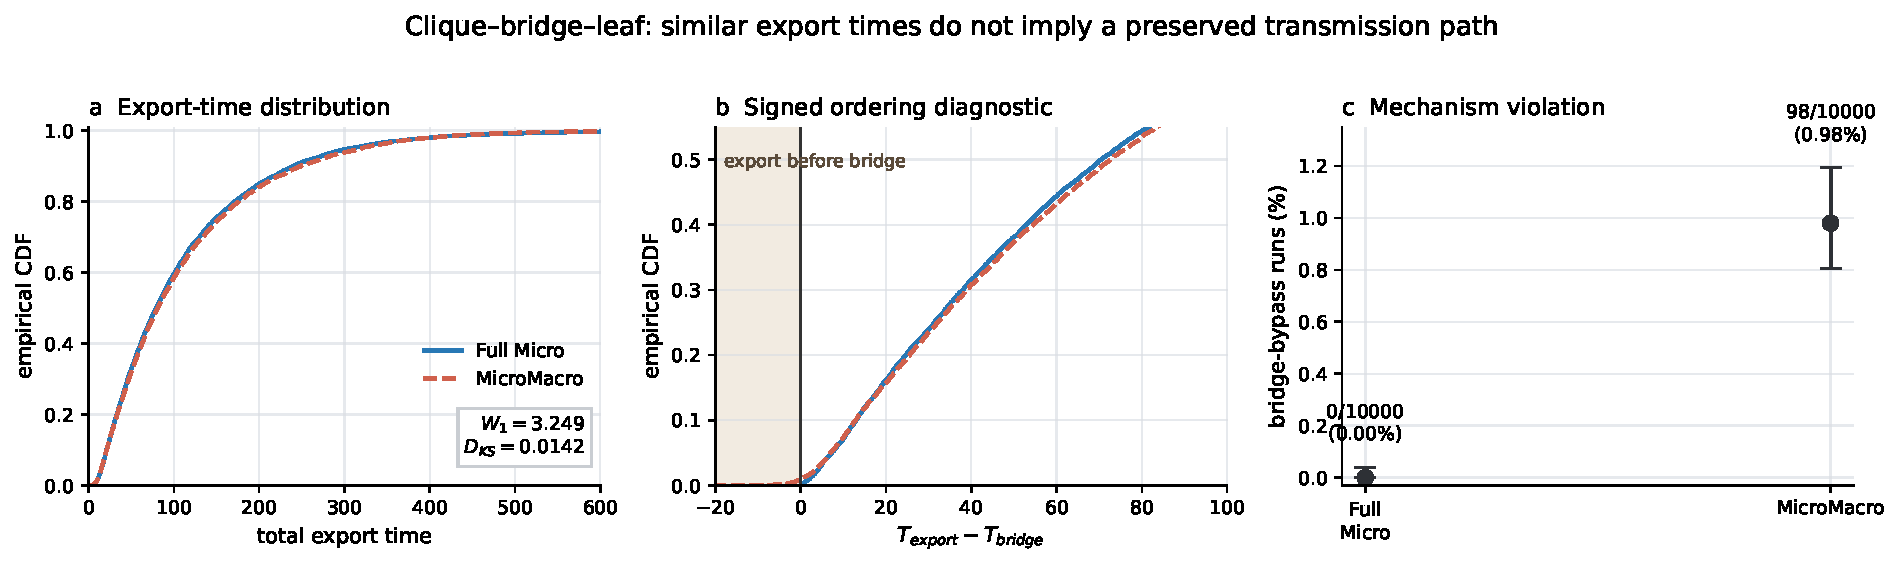
\includegraphics[width=\linewidth]{Images/clique_leaf/clique_leaf_endpoint_and_mechanism.pdf}
\caption{Clique--leaf benchmark ($n=100$, $k=2$, $\beta=0.005$, 10\,000 runs per model). (a) Empirical CDFs of the export time. (b) Empirical CDFs of $T_{\mathrm{export}}-T_B$; negative values (shaded) are exports before any bridge node is infected. (c) Percentage of such bridge-bypass runs with 95\% intervals. ``Full Micro'' denotes \Full{} and ``MicroMacro'' denotes \TS{}.}
\label{fig:clique_leaf}
\end{figure}

\subsection{Single export from connected random sources}
\label{sec:res_source}

\emph{As internal paths lengthen, bridge bypass becomes common and the aggregate export becomes early, as predicted by Proposition~\ref{prop:ordering}.} Figure~\ref{fig:source_sweep} shows the source--leaf sweep. Mean bridge activation times were similar in the two models, within 7\% at every ASPL (e.g.\ 1165 and 1136 at ASPL 6, $k=1$), as expected from identical local dynamics before the export. In \Full{} with $k=1$, the wait after bridge activation stayed at 322--359 at every ASPL, consistent with $\mathrm{Exp}(\beta)$ with mean 333. In \TS{}, the signed interval $T_{\mathrm{export}}-T_B$ ($k=1$) shrank from about 340 in dense sources to 207--295 at ASPL $\ge5$, because aggregate hazard accumulated before the true bridge became infectious.

\begin{figure}[tbp]
\centering
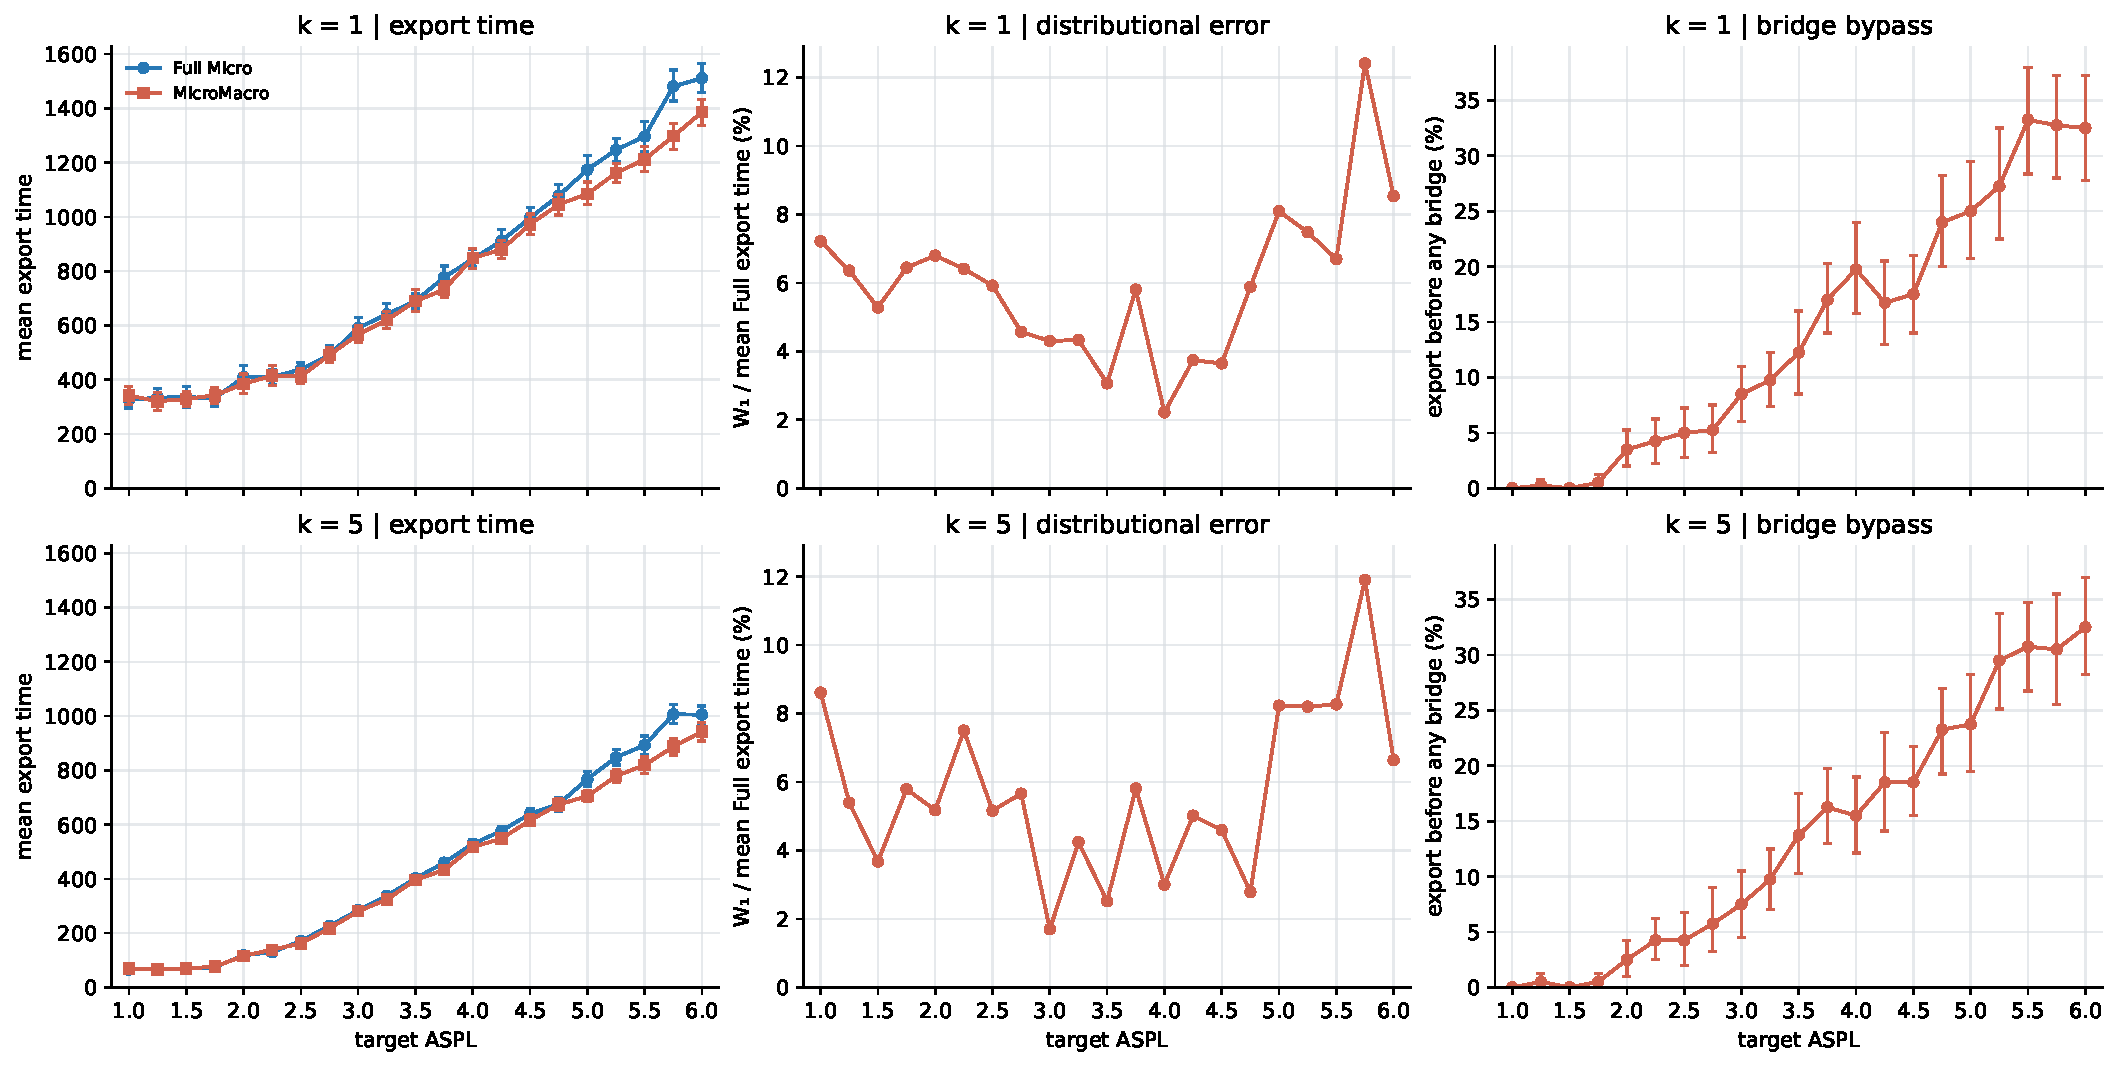
\includegraphics[width=\linewidth]{Images/fig_aspl_export_fidelity.pdf}
\caption{Source--leaf sweep: $n=1000$, $\beta=0.003$, $k=1$ (top) and $k=5$ (bottom), 400 matched runs per point. Left: mean export time. Centre: relative Wasserstein distance $\eW$ of the export-time distributions. Right: percentage of \TS{} exports that precede the first bridge infection; \Full{} had none. Whiskers are 95\% block-bootstrap intervals. ``Full Micro'' denotes \Full{} and ``Production MicroMacro'' denotes \TS{}.}
\label{fig:source_sweep}
\end{figure}

The bypass fraction rose from at most 0.5\% for ASPL $\le1.75$ to 19.75\% (95\% interval 15.8--24.0\%) at ASPL 4 with $k=1$, and to 32.5\% for both widths at ASPL 6. The mean export shift was resolved, with intervals excluding zero, for both widths at every ASPL $\ge5$. Its values ranged from $-6.2\%$ to $-12.4\%$; at ASPL 6 they were $-8.3\%$ ($[-13.1,-3.5]$) for $k=1$ and $-6.2\%$ ($[-10.3,-2.3]$) for $k=5$. Below ASPL 5, a shift was resolved only for $k=5$ at ASPL 3.75, 4.25 and 4.5 (between $-3.7\%$ and $-5.8\%$). No positive shift was resolved anywhere in the sweep, in agreement with the direction predicted by Proposition~\ref{prop:ordering}.

The irregular centre panel requires care. For nearly exponential export times and $R=400$ runs per model, the expected $\eW$ of two samples from the same law is about $\sqrt{\pi/R}\approx9\%$ (Appendix~\ref{app:floor}). The values of 3.7--8.6\% observed for ASPL $\le1.75$ are therefore consistent with pure sampling variability. Single-export distances should thus be read together with the mean shift and its interval. Bypass, by contrast, is zero in \Full{} by construction, so any observed bypass is a genuine discrepancy. At ASPL 4 it affects one fifth of the exports while the export-time distributions remain close.

\subsection{Repeated crossings through a chain of cliques}
\label{sec:res_cliques}

\emph{When internal spread is fast, close agreement survives nine successive aggregate crossings.} In the chain of ten 1000-node cliques with $k=1$, the median terminal arrival was 2785 in \Full{} and 2877 in \TS{}, and $\eW=3.34\%$ (Figure~\ref{fig:chain_cliques}). The permutation floor of this cell was 5.1\% ($p=0.32$), so the two terminal distributions are statistically indistinguishable. The CDFs cross, so the difference is not a fixed delay. A 1000-node clique saturates on average within $2H_{999}/(\beta n)\approx5$ time units, compared with a mean edge-crossing time of 333 ($\rho=0.002$). The aggregate rate therefore differs from the exact one only during a negligible fraction of each crossing.

\begin{figure}[tbp]
\centering
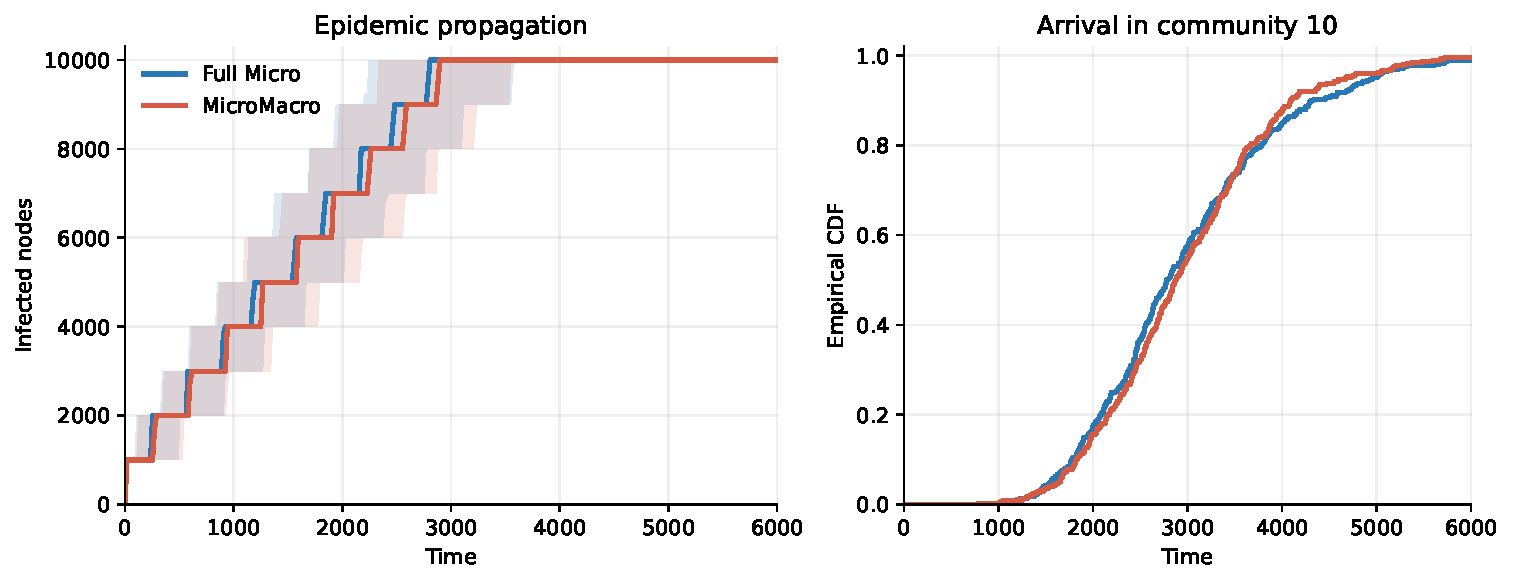
\includegraphics[width=\linewidth]{Images/chain_cliques/chain_cliques_n1000_k1_propagation_cdf_random_initial.pdf}
\caption{Chain of ten 1000-node cliques with one edge between consecutive cliques ($k=1$, $\beta=0.003$, 400 runs per model). Left: pointwise median number of infected nodes with interquartile bands. Right: empirical CDF of the arrival time in the tenth community ($T_9$). Four \Full{} and two \TS{} arrivals lie beyond the displayed range; all were observed.}
\label{fig:chain_cliques}
\end{figure}

\subsection{Chains of random communities}
\label{sec:res_chain_random}

\emph{Sparse, long-path communities produce systematically early arrivals whose relative size is stable along the chain while the absolute lead accumulates.} Figure~\ref{fig:chain_heatmap} shows the cumulative arrival times in chains of 1000-node communities. For target ASPL 2--3, terminal $\eW$ was 1.4--2.5\%, close to its sampling floor. At ASPL 6, \TS{} reached the last community earlier by 13.9\% in median for $k=1$ and by 10.7\% for $k=5$ ($\eW=13.6\%$ and 10.9\%). Along the ASPL-5 row with $k=1$, the relative median lead was about 10\% at both the first and the last community, while its absolute size grew from about 107 to 1018 time units. A constant relative error along a chain therefore means a growing absolute error at distant communities. The positive first-column values in the clique row ($+12.6\%$ and $+11.5\%$) are not resolved: for $k=1$, the first-crossing mean shift is $+4.9\%$ with a 95\% interval of $[-8.0,18.3]\%$. Single-crossing distances also have a larger sampling floor than cumulative ones.

\begin{figure}[tbp]
\centering
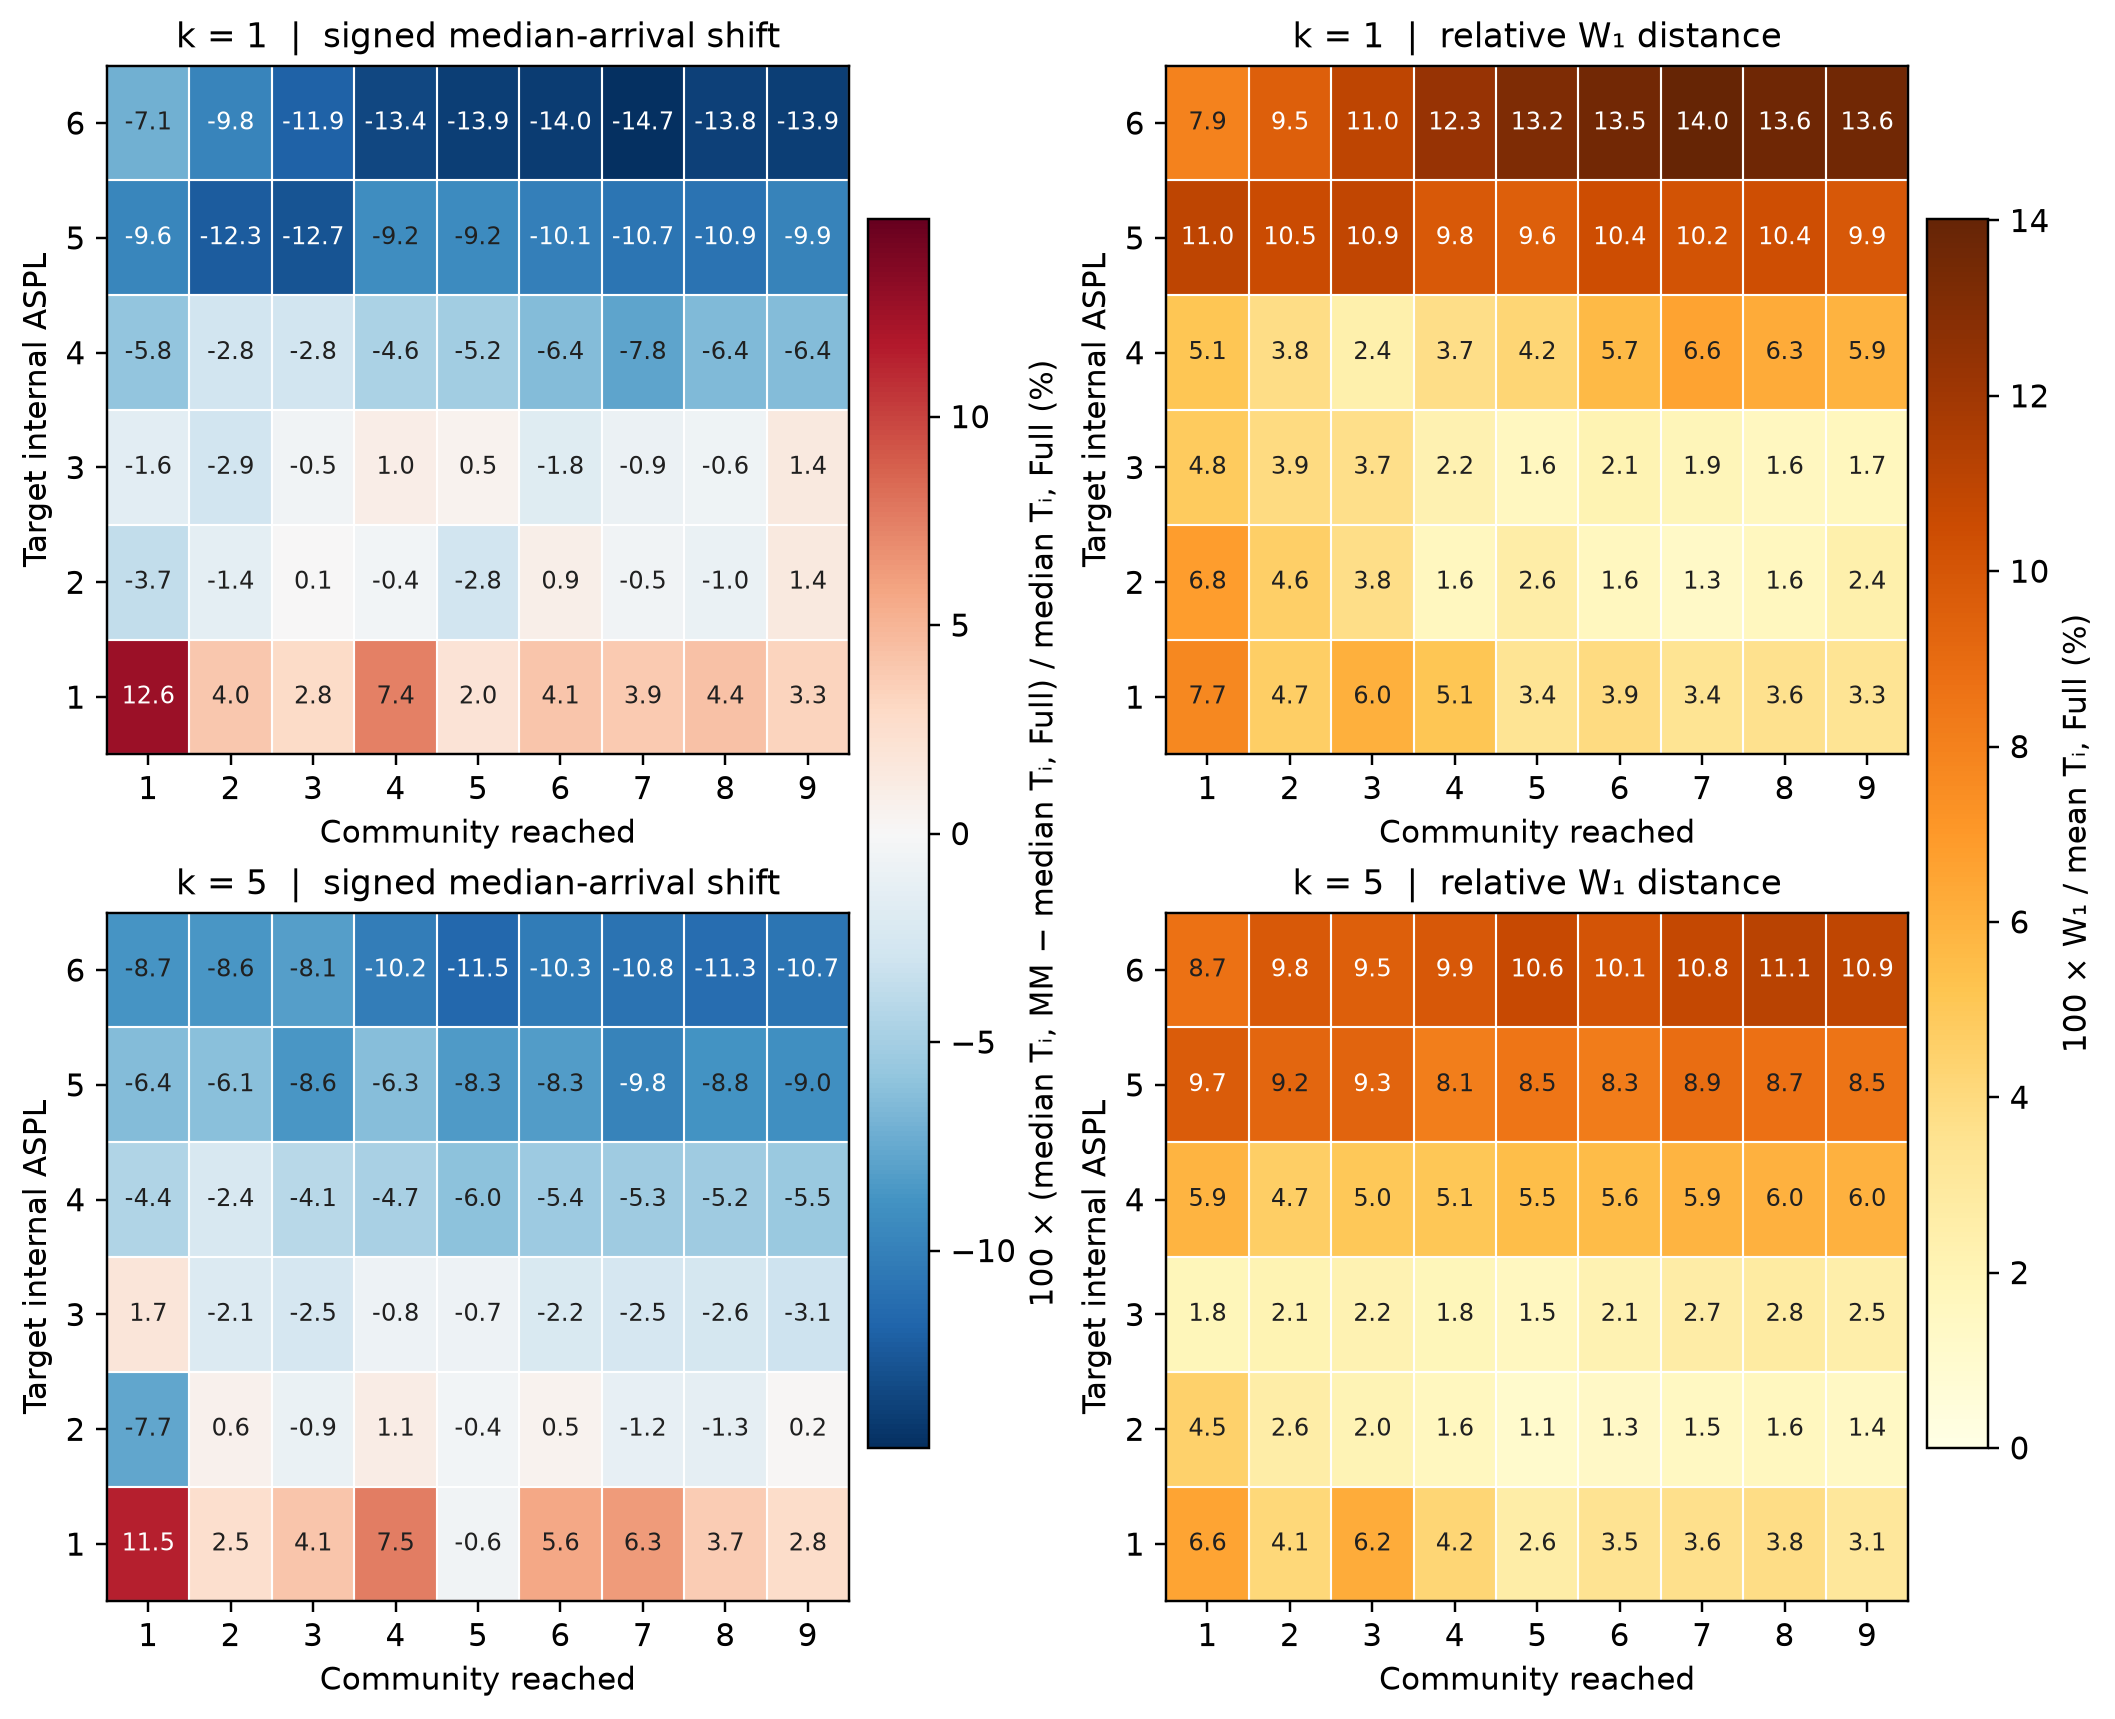
\includegraphics[width=0.82\linewidth]{Images/aspl_chain/aspl_chain_median_arrival_error_map_labeled.png}
\caption{Cumulative arrival accuracy in ten-community chains with $n=1000$, by target ASPL (rows) and community reached ($c=1,\dots,9$, columns), for $k=1$ (top) and $k=5$ (bottom). Left: relative median shift $b_c$ (negative: \TS{} earlier). Right: relative Wasserstein distance. Each cell uses 400 matched runs; no uncertainty is shown (see Figure~\ref{fig:accuracy_map} for the terminal arrivals).}
\label{fig:chain_heatmap}
\end{figure}

\subsection{Community size and interface width}
\label{sec:res_size}

\emph{The same internal path length is much less favourable in small communities.} Figure~\ref{fig:accuracy_map} reports the terminal discrepancy for all 48 configurations of the size sweep. The permutation floor ranged from 1.6\% to 5.9\%. In the 16 configurations with ASPL $\le2$, $\eW$ was 1.1--4.4\%, and in 14 of them it was not distinguishable from the floor at the 5\% level. In 31 of the 32 configurations with ASPL $\ge3$, $\eW$ exceeded the floor ($p<0.01$), and the median shift was negative with a block-bootstrap interval excluding zero. The exception was $n=1000$, ASPL 3, $k=1$, with $\eW=1.7\%$. At a fixed ASPL $\ge3$, the discrepancy decreased monotonically with community size for both interface widths. At ASPL 6, $\eW$ fell from 41.3\% for $n=50$ to 13.6\% for $n=1000$ with $k=1$, and from 32.4\% to 10.9\% with $k=5$. Wider interfaces reduced the discrepancy in sparse communities but did not remove it. The fraction of \TS{} crossings that preceded infection of any bridge node of the source community rose from 0.1--2.3\% at ASPL 1 to 30--52\% at ASPL 6.

\begin{figure}[tbp]
\centering
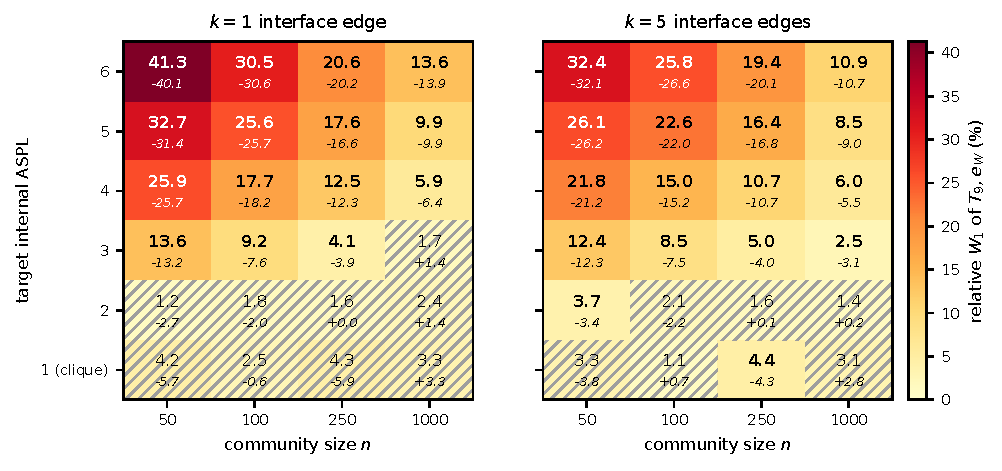
\includegraphics[width=\linewidth]{Images/twoscale/fig_accuracy_map.pdf}
\caption{Terminal-arrival accuracy in ten-community chains for all 48 configurations of the size sweep. Colour and bold numbers: relative Wasserstein distance $\eW$ of $T_9$ (\%). Italic numbers: relative median shift $b_9$ (\%; negative means \TS{} earlier). Hatched cells: $\eW$ not distinguishable from its within-pair permutation floor ($p\ge0.05$). Each cell: 400 matched runs.}
\label{fig:accuracy_map}
\end{figure}

\subsection{A single time-scale ratio organises the discrepancy}
\label{sec:res_descriptor}

\emph{Expressed through $\rho=\beta\sigma_T$, the results of all sizes, structures and interface widths collapse onto one curve.} We computed $\sigma_T$ in each configuration as the standard deviation of node infection times within each source community of the \Full{} runs, averaged over communities and runs. Figure~\ref{fig:descriptor}(a,b) plots the terminal $\eW$ and $b_9$ against $\rho$. The rank correlation between $\eW$ and $\rho$ was 0.92 over all 48 configurations and 0.98 over the 32 configurations with ASPL $\ge3$; the corresponding values for target ASPL were 0.82 and 0.67. In the 18 configurations with $\rho<0.25$, $\eW\le4.4\%$, and 15 were indistinguishable from the permutation floor. All 30 configurations with $\rho\ge0.25$ were resolved. For $\rho\ge0.3$, a log--log fit gave $\eW\approx15\rho\,\%$ (slope 1.03; median relative deviation 8\%, maximum 41\%), and $b_9\approx-\eW$, i.e.\ the discrepancy was almost entirely an early shift. We also examined two alternative scalings: $\beta\sqrt{k}\sigma_T$, suggested by~\eqref{eq:hazard_variance}, and the mean time from a community's first infection to infection of its first bridge node, multiplied by $\beta k$. Both separated the two interface widths more than $\rho$ did.

\begin{figure}[tbp]
\centering
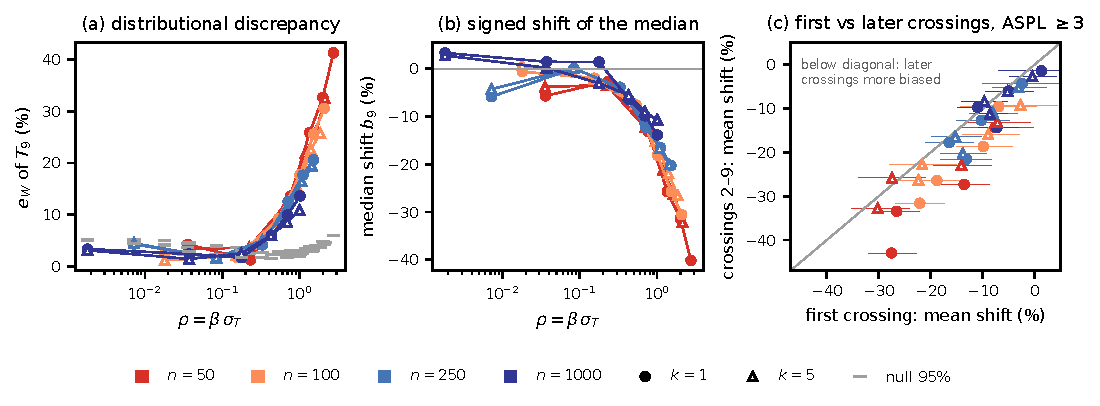
\includegraphics[width=\linewidth]{Images/twoscale/fig_descriptor.pdf}
\caption{(a) Relative Wasserstein distance and (b) relative median shift of the terminal arrival against $\rho=\beta\sigma_T$, for all 48 chain configurations (colours: community size; filled circles: $k=1$; open triangles: $k=5$; lines connect ASPL 1--6 at fixed $n$ and $k$). Grey ticks in (a): 95th percentile of the within-pair permutation floor of each configuration. (c) Local mean shift of the first crossing against that of crossings 2--9, for configurations with ASPL $\ge3$, with 95\% block-bootstrap intervals of the first-crossing shift.}
\label{fig:descriptor}
\end{figure}

Figure~\ref{fig:descriptor}(c) separates the crossings. By Remark~\ref{rem:placement}, the first crossing in our design is subject only to source-side and numerical mechanisms, whereas later crossings are also subject to placement after the first import and to surplus imports. For $k=1$, later crossings were more strongly biased than the first in 15 of the 16 configurations with ASPL $\ge3$. The difference was resolved in 9 of them, including all four sizes at ASPL 6; for example, $-27.5\%$ for the first crossing against $-42.9\%$ for crossings 2--9 at $n=50$. For $k=5$, the difference was smaller (14 of 16 point estimates negative, 3 resolved). This dependence on $k$ is what interface exhaustion predicts: a single physical edge permits one crossing, whereas five edges permit up to five, so surplus aggregate imports matter less. Because seeds are shared between configurations, we regard this pattern as supporting rather than conclusive evidence. A direct count of surplus imports would require event-type logs that were not stored.

%======================================================================
\section{Discussion}
\label{sec:discussion}

\subsection{Practical guidance}

The results suggest a simple procedure for deciding whether aggregate coupling is adequate.

\paragraph{Decide which observable matters.}
For the timing of spread between communities, the two-scale simulator can be accurate. For transmission routes, it cannot be trusted. Up to half of its crossings in sparse communities, and a fifth of exports even where export-time distributions agreed, occurred before any true bridge node was infected. Questions that depend on bridge nodes, such as targeting interventions at the individuals who connect communities or attributing an outbreak to a source, require boundary information that the aggregate interface does not contain.

\paragraph{Estimate the time-scale ratio.}
Compute $\rho=\beta_{\mathrm{out}}\sigma_T$. Since $\sigma_T$ describes spread within a single community, it can in principle be estimated from the local engines alone, by simulating an isolated community from a uniformly placed seed. We computed it from the reference runs and have not tested this local estimate. In our benchmarks, terminal arrivals were statistically indistinguishable for $\rho\lesssim0.25$. For $0.3\lesssim\rho\lesssim3$, \TS{} arrived early by roughly $15\rho\%$. This rule is an empirical summary of one family of synthetic networks and parameters, not a general error law.

\paragraph{Check absolute as well as relative errors.}
Along a chain, the relative discrepancy was nearly constant, so the absolute lead at distant communities grew in proportion to the travel time. For intervention timing at a specific destination, the absolute discrepancy at that destination is the relevant quantity.

\paragraph{Calibrate distances against sampling variability.}
With a few hundred runs per model, distances of a few percent between arrival-time distributions are expected even between identical models (Appendix~\ref{app:floor}). Permutation baselines or analytical floors should accompany such comparisons.

\subsection{Computational cost}
\label{sec:disc_cost}

The benchmarks were designed for accuracy assessment, so their explicit interfaces contain at most five edges and the full reference is cheap. In this regime, aggregation removes almost no work, and the cost of grid synchronisation dominates. The median wall-clock time per replicate of the Python implementations ranged from 0.04--0.07\,s (\Full{}) and 0.6--31\,s (\TS{}) for $n=50$ to 8.6--18\,s and 6.7--124\,s for $n=1000$. For $n=1000$, the ratio of the two medians ranged from 0.76 (ASPL 2, $k=5$) to 6.9 (ASPL 6, $k=1$). Two conclusions follow. First, in settings where the full network is known and small, \Full{} should be preferred. Second, the overhead of the two-scale method stems from the black-box scheduler rather than from aggregation. An event-driven scheduler that integrates the piecewise-constant hazard exactly (Section~\ref{sec:timing}) would remove both this overhead and the synchronisation error. Computational gains are expected when inter-community contacts are numerous or unavailable, which is the setting the method is intended for \citep{kuryliak2025towards}; quantifying them is left to future work.

\subsection{Limitations}

The experiments use SI dynamics. With recovery, bridge nodes can stop transmitting while the community-wide fraction remains positive, and the aggregate rate may then also overestimate exports late in a local outbreak. All networks are synthetic, the macro-topology is a chain, and internal and external per-edge rates are equal. Interfaces were placed at random, which by Remark~\ref{rem:placement} neutralises placement error for first imports. Structured interfaces, for example with bridges at hubs or with incoming and outgoing bridges far apart, may behave differently. The synchronisation step was not varied, so the numerical component of the discrepancy was not isolated; Proposition~\ref{prop:surrogate} provides a direct way to do so. Finally, $\rho$ was evaluated with reference runs and chosen among a small number of candidate scalings; its predictive value for other network families remains to be tested.

\subsection{Possible extensions}

The analysis points to modifications that use only aggregate information. Interface exhaustion can be represented by limiting the number of imports per bundle to its number of channels, which is known whenever $W_{ij}$ counts edges, or by reducing $\lambda_{ij}$ as this capacity is consumed. When partial boundary information is available, $\ibar_i$ in~\eqref{eq:macro_rate} can be replaced by the infected fraction among known bridge nodes. Placement can then be restricted to known receiving endpoints. Each such variant can be evaluated against \Full{} and against exact simulation on $\tilde G$, which separates modelling from numerical error.

%======================================================================
\section{Conclusions}
\label{sec:conclusions}

The two-scale method couples exact local Gillespie engines through aggregate inter-community hazards. In its ideal form, it is exact simulation on a surrogate network in which every interface is smeared uniformly over all pairs of nodes. This identifies what the method loses: the state of the actual bridge nodes, the location of imports and the finite capacity of thin interfaces. For randomly placed interfaces, it also implies that aggregate export clocks are stochastically early. In controlled comparisons with full-network Gillespie simulation, terminal arrival-time distributions were statistically indistinguishable when infection spread through communities quickly relative to the time needed to cross an interface edge. As the internal timing spread approached and exceeded that crossing time, the two-scale simulator arrived systematically early, by up to 40\% in small sparse communities. The ratio $\rho=\beta\sigma_T$ organised these results across community sizes, internal structures and interface widths. Close timing never guaranteed admissible transmission routes. The method is therefore a reasonable tool for propagation-time questions when $\rho$ is small. It is not suited to questions about individual transmission routes, or to sparse communities with long internal paths unless the interface is refined.

%======================================================================
\appendix

\section{Clique formulas and verification}
\label{app:clique}

Consider an $n$-node clique with SI dynamics, per-edge rate $\beta$, a uniformly placed seed and a uniformly placed set of $k$ bridge nodes. When $m$ nodes are infected, the next internal infection occurs at rate $\beta m(n-m)$, independently of which nodes are infected, and the infected set is a uniform $m$-subset. The probability that none of the first $m$ infected nodes is a bridge is $\binom{n-k}{m}/\binom{n}{m}$, hence
\begin{equation}
\label{eq:clique_TB}
\mathbb{E}[T_B]=\sum_{m=1}^{n-k}\frac{\binom{n-k}{m}}{\binom{n}{m}}\frac{1}{\beta m(n-m)},
\qquad
\mathbb{E}[T_B]=\frac{H_{n-1}}{\beta n}\ \ (k=1),
\end{equation}
where $H_{n-1}$ is the harmonic number; the case of a bridge seed ($T_B=0$) is included. For $k=1$, the export time in \Full{} is $T_B$ plus an independent $\Exp(\beta)$ waiting time. The expected time to infect the whole clique is $2H_{n-1}/(\beta n)$. Table~\ref{tab:verification} compares~\eqref{eq:clique_TB} with the first community of the clique chains.

\begin{table}[tbp]
\centering
\caption{Verification of the reference simulator on the first community of the clique chains ($\beta=0.003$, 400 runs per cell): mean bridge-activation time and, for $k=1$, mean wait after activation (exact value $1/\beta=333.3$). Values are mean $\pm$ standard error.}
\label{tab:verification}
\small
\begin{tabular}{rrrrr}
\toprule
$n$ & $k$ & $\mathbb{E}[T_B]$, Eq.~\eqref{eq:clique_TB} & \Full{} mean $T_B$ & \Full{} wait after $T_B$\\
\midrule
50 & 1 & 29.86 & $29.72\pm0.71$ & $354.0\pm16.9$\\
100 & 1 & 17.26 & $17.05\pm0.38$ & $326.5\pm17.0$\\
250 & 1 & 8.13 & $7.84\pm0.15$ & $347.4\pm16.6$\\
1000 & 1 & 2.49 & $2.51\pm0.04$ & $353.8\pm17.9$\\
50 & 5 & 15.97 & $15.96\pm0.55$ & --\\
100 & 5 & 10.31 & $9.64\pm0.29$ & --\\
250 & 5 & 5.35 & $5.16\pm0.12$ & --\\
1000 & 5 & 1.80 & $1.77\pm0.03$ & --\\
\bottomrule
\end{tabular}
\end{table}

\section{Sampling floor of the Wasserstein distance}
\label{app:floor}

Let $F_R$ and $G_R$ be empirical CDFs of two independent samples of size $R$ from the same continuous law $F$. Then $W_1=\int|F_R-G_R|\,dx$, and $\sqrt{R}\,(F_R-G_R)$ is approximately $\sqrt{2}$ times a Brownian bridge evaluated at $F(x)$ \citep{delbarrio1999}. Since $\mathbb{E}|B(u)|=\sqrt{2u(1-u)/\pi}$ for a Brownian bridge $B$,
\[
\mathbb{E}[W_1]\approx\frac{2}{\sqrt{\pi R}}\int\sqrt{F(x)\bigl(1-F(x)\bigr)}\,dx .
\]
For an exponential law with mean $\mu$, the integral equals $\mu\pi/2$, so that $\mathbb{E}[W_1]/\mu\approx\sqrt{\pi/R}$, which is 8.9\% for $R=400$ and 1.8\% for $R=10\,000$. Arrival times that are sums of several crossings are less dispersed relative to their mean, and their floor is correspondingly lower; the permutation floors of the chain configurations ranged from 1.6\% to 5.9\%.

\section{Reproducibility details}
\label{app:repro}

Seeds are derived deterministically from the experiment parameters. Each \TS{} engine draws from a private pseudorandom stream; midpoint probes copy the stream state of their engine and do not advance it. Two \Full{} runs ($n=50$, ASPL 6, $k=1$) had not reached the tenth community by $T=30\,000$. They were rerun to $T=40\,000$ with the same graphs, initial nodes and event seeds. Their event histories up to 30\,000 were verified to match the saved runs, and their terminal arrivals occurred at about 31\,059 and 31\,007. No horizon value was substituted for an unobserved event. The permutation and bootstrap analyses of the chain configurations, the descriptor $\sigma_T$ and Figures~\ref{fig:accuracy_map}--\ref{fig:descriptor} were computed from the saved runs by the scripts \path{extrascripts/analysis/smpt_twoscale_paper_metrics.py} and \path{extrascripts/visualization/smpt_twoscale_paper_figures.py}.

%======================================================================
\section*{CRediT authorship contribution statement}
\textbf{Yulian Kuryliak:} Conceptualization, Methodology, Software, Investigation, Formal analysis, Visualization, Writing -- original draft. \textbf{Michael T. M. Emmerich:} Conceptualization, Methodology, Supervision, Writing -- review \& editing. [Authors to confirm.]

\section*{Declaration of competing interest}
The authors declare that they have no known competing financial interests or personal relationships that could have appeared to influence the work reported in this paper.

\section*{Funding}
[Funding information to be added by the authors.]

\section*{Data availability}
The simulation code, saved simulation outputs and analysis scripts are available from the corresponding author on reasonable request. [Replace with a repository DOI if the data are deposited.]

\section*{Declaration of generative AI and AI-assisted technologies in the manuscript preparation process}
During the preparation of this work the authors used [name of tool or service] in order to [reason]. After using this tool or service, the authors reviewed and edited the content as needed and take full responsibility for the content of the published article. [Authors to complete.]

\bibliographystyle{cas-model2-names}
\bibliography{twoscale_references}

\end{document}
